\documentclass[twoside]{book}

% Packages required by doxygen
\usepackage{fixltx2e}
\usepackage{calc}
\usepackage{doxygen}
\usepackage[export]{adjustbox} % also loads graphicx
\usepackage{graphicx}
\usepackage[utf8]{inputenc}
\usepackage{makeidx}
\usepackage{multicol}
\usepackage{multirow}
\PassOptionsToPackage{warn}{textcomp}
\usepackage{textcomp}
\usepackage[nointegrals]{wasysym}
\usepackage[table]{xcolor}

% Font selection
\usepackage[T1]{fontenc}
\usepackage[scaled=.90]{helvet}
\usepackage{courier}
\usepackage{amssymb}
\usepackage{sectsty}
\renewcommand{\familydefault}{\sfdefault}
\allsectionsfont{%
  \fontseries{bc}\selectfont%
  \color{darkgray}%
}
\renewcommand{\DoxyLabelFont}{%
  \fontseries{bc}\selectfont%
  \color{darkgray}%
}
\newcommand{\+}{\discretionary{\mbox{\scriptsize$\hookleftarrow$}}{}{}}

% Page & text layout
\usepackage{geometry}
\geometry{%
  a4paper,%
  top=2.5cm,%
  bottom=2.5cm,%
  left=2.5cm,%
  right=2.5cm%
}
\tolerance=750
\hfuzz=15pt
\hbadness=750
\setlength{\emergencystretch}{15pt}
\setlength{\parindent}{0cm}
\setlength{\parskip}{3ex plus 2ex minus 2ex}
\makeatletter
\renewcommand{\paragraph}{%
  \@startsection{paragraph}{4}{0ex}{-1.0ex}{1.0ex}{%
    \normalfont\normalsize\bfseries\SS@parafont%
  }%
}
\renewcommand{\subparagraph}{%
  \@startsection{subparagraph}{5}{0ex}{-1.0ex}{1.0ex}{%
    \normalfont\normalsize\bfseries\SS@subparafont%
  }%
}
\makeatother

% Headers & footers
\usepackage{fancyhdr}
\pagestyle{fancyplain}
\fancyhead[LE]{\fancyplain{}{\bfseries\thepage}}
\fancyhead[CE]{\fancyplain{}{}}
\fancyhead[RE]{\fancyplain{}{\bfseries\leftmark}}
\fancyhead[LO]{\fancyplain{}{\bfseries\rightmark}}
\fancyhead[CO]{\fancyplain{}{}}
\fancyhead[RO]{\fancyplain{}{\bfseries\thepage}}
\fancyfoot[LE]{\fancyplain{}{}}
\fancyfoot[CE]{\fancyplain{}{}}
\fancyfoot[RE]{\fancyplain{}{\bfseries\scriptsize Generated by Doxygen }}
\fancyfoot[LO]{\fancyplain{}{\bfseries\scriptsize Generated by Doxygen }}
\fancyfoot[CO]{\fancyplain{}{}}
\fancyfoot[RO]{\fancyplain{}{}}
\renewcommand{\footrulewidth}{0.4pt}
\renewcommand{\chaptermark}[1]{%
  \markboth{#1}{}%
}
\renewcommand{\sectionmark}[1]{%
  \markright{\thesection\ #1}%
}

% Indices & bibliography
\usepackage{natbib}
\usepackage[titles]{tocloft}
\setcounter{tocdepth}{3}
\setcounter{secnumdepth}{5}
\makeindex

% Hyperlinks (required, but should be loaded last)
\usepackage{ifpdf}
\ifpdf
  \usepackage[pdftex,pagebackref=true]{hyperref}
\else
  \usepackage[ps2pdf,pagebackref=true]{hyperref}
\fi
\hypersetup{%
  colorlinks=true,%
  linkcolor=blue,%
  citecolor=blue,%
  unicode%
}

% Custom commands
\newcommand{\clearemptydoublepage}{%
  \newpage{\pagestyle{empty}\cleardoublepage}%
}

\usepackage{caption}
\captionsetup{labelsep=space,justification=centering,font={bf},singlelinecheck=off,skip=4pt,position=top}

%===== C O N T E N T S =====

\begin{document}

% Titlepage & ToC
\hypersetup{pageanchor=false,
             bookmarksnumbered=true,
             pdfencoding=unicode
            }
\pagenumbering{alph}
\begin{titlepage}
\vspace*{7cm}
\begin{center}%
{\Large Trabalho de Implementação II -\/ identificação de prefixos e indexação de dicionários }\\
\vspace*{1cm}
{\large Generated by Doxygen 1.8.13}\\
\end{center}
\end{titlepage}
\clearemptydoublepage
\pagenumbering{roman}
\tableofcontents
\clearemptydoublepage
\pagenumbering{arabic}
\hypersetup{pageanchor=true}

%--- Begin generated contents ---
\chapter{Class Index}
\section{Class List}
Here are the classes, structs, unions and interfaces with brief descriptions\+:\begin{DoxyCompactList}
\item\contentsline{section}{\hyperlink{classstructures_1_1Parser}{structures\+::\+Parser} }{\pageref{classstructures_1_1Parser}}{}
\item\contentsline{section}{\hyperlink{classstructures_1_1Trie}{structures\+::\+Trie} \\*Classe da \hyperlink{classstructures_1_1Trie}{Trie}. Estrutura de Dados responsável pela indexação das palavras }{\pageref{classstructures_1_1Trie}}{}
\end{DoxyCompactList}

\chapter{File Index}
\section{File List}
Here is a list of all files with brief descriptions\+:\begin{DoxyCompactList}
\item\contentsline{section}{\hyperlink{linked__queue_8h}{linked\+\_\+queue.\+h} }{\pageref{linked__queue_8h}}{}
\item\contentsline{section}{\hyperlink{linked__stack_8h}{linked\+\_\+stack.\+h} }{\pageref{linked__stack_8h}}{}
\item\contentsline{section}{\hyperlink{main_8cpp}{main.\+cpp} \\*Primeiro trabalho da disciplina de Estrutura de Dados(\+I\+N\+E5408) }{\pageref{main_8cpp}}{}
\end{DoxyCompactList}

\chapter{Class Documentation}
\hypertarget{classstructures_1_1Parser}{}\section{structures\+:\+:Parser Class Reference}
\label{classstructures_1_1Parser}\index{structures\+::\+Parser@{structures\+::\+Parser}}
\subsection*{Public Member Functions}
\begin{DoxyCompactItemize}
\item 
\hyperlink{classstructures_1_1Parser_a62344223eabcf9cd5e2cf6f6b5ea2139}{Parser} (std\+::string \hyperlink{classstructures_1_1Parser_ac5ccd294f3176bcac3f1de2045e523ef}{file\+Name})
\begin{DoxyCompactList}\small\item\em Construtor do \hyperlink{classstructures_1_1Parser}{Parser}. \end{DoxyCompactList}\item 
std\+::string \hyperlink{classstructures_1_1Parser_a0c3fe341a7d74b1db953cc19eeba7062}{get\+Dic\+Text} ()
\begin{DoxyCompactList}\small\item\em Armazenamento do texto do arquivo do dicionário. \end{DoxyCompactList}\item 
void \hyperlink{classstructures_1_1Parser_a4cab45335029ece42ba0d79263621ace}{parsing} (std\+::string dic\+Text, \hyperlink{classstructures_1_1Trie}{structures\+::\+Trie} trie)
\begin{DoxyCompactList}\small\item\em Extração das palavras, posições e comprimentos. \end{DoxyCompactList}\end{DoxyCompactItemize}
\subsection*{Public Attributes}
\begin{DoxyCompactItemize}
\item 
std\+::string \hyperlink{classstructures_1_1Parser_ac5ccd294f3176bcac3f1de2045e523ef}{file\+Name}
\end{DoxyCompactItemize}


\subsection{Detailed Description}
Classe para o \hyperlink{classstructures_1_1Parser}{Parser}. 

\subsection{Constructor \& Destructor Documentation}
\mbox{\Hypertarget{classstructures_1_1Parser_a62344223eabcf9cd5e2cf6f6b5ea2139}\label{classstructures_1_1Parser_a62344223eabcf9cd5e2cf6f6b5ea2139}} 
\index{structures\+::\+Parser@{structures\+::\+Parser}!Parser@{Parser}}
\index{Parser@{Parser}!structures\+::\+Parser@{structures\+::\+Parser}}
\subsubsection{\texorpdfstring{Parser()}{Parser()}}
{\footnotesize\ttfamily structures\+::\+Parser\+::\+Parser (\begin{DoxyParamCaption}\item[{std\+::string}]{file\+Name }\end{DoxyParamCaption})\hspace{0.3cm}{\ttfamily [inline]}}



Construtor do \hyperlink{classstructures_1_1Parser}{Parser}. 


\begin{DoxyParams}{Parameters}
{\em file\+Name} & Nome do arquivo do dicionário. \\
\hline
\end{DoxyParams}


\subsection{Member Function Documentation}
\mbox{\Hypertarget{classstructures_1_1Parser_a0c3fe341a7d74b1db953cc19eeba7062}\label{classstructures_1_1Parser_a0c3fe341a7d74b1db953cc19eeba7062}} 
\index{structures\+::\+Parser@{structures\+::\+Parser}!get\+Dic\+Text@{get\+Dic\+Text}}
\index{get\+Dic\+Text@{get\+Dic\+Text}!structures\+::\+Parser@{structures\+::\+Parser}}
\subsubsection{\texorpdfstring{get\+Dic\+Text()}{getDicText()}}
{\footnotesize\ttfamily std\+::string structures\+::\+Parser\+::get\+Dic\+Text (\begin{DoxyParamCaption}{ }\end{DoxyParamCaption})\hspace{0.3cm}{\ttfamily [inline]}}



Armazenamento do texto do arquivo do dicionário. 

\begin{DoxyReturn}{Returns}
O texto do dicionário. 
\end{DoxyReturn}
\mbox{\Hypertarget{classstructures_1_1Parser_a4cab45335029ece42ba0d79263621ace}\label{classstructures_1_1Parser_a4cab45335029ece42ba0d79263621ace}} 
\index{structures\+::\+Parser@{structures\+::\+Parser}!parsing@{parsing}}
\index{parsing@{parsing}!structures\+::\+Parser@{structures\+::\+Parser}}
\subsubsection{\texorpdfstring{parsing()}{parsing()}}
{\footnotesize\ttfamily void structures\+::\+Parser\+::parsing (\begin{DoxyParamCaption}\item[{std\+::string}]{dic\+Text,  }\item[{\hyperlink{classstructures_1_1Trie}{structures\+::\+Trie}}]{trie }\end{DoxyParamCaption})\hspace{0.3cm}{\ttfamily [inline]}}



Extração das palavras, posições e comprimentos. 

Primeiramente ocorrerá a extração da palavra através da procura pelos caracteres \textquotesingle{}\mbox{]}\textquotesingle{} (begin) e \textquotesingle{}\mbox{[}\textquotesingle{} (end\+Word). Posteriormente, será buscada o índice do caractere de quebra de linha (end). O comprimento será a diferença entre o índice begin e o end, enquanto que a posição será o próprio begin. A atualização do índice begin é realizada em saltos conforme o comprimento das linhas do dicionário. Por fim, a palavra será inserida na \hyperlink{classstructures_1_1Trie}{Trie}.


\begin{DoxyParams}{Parameters}
{\em dic\+Text} & O texto do dicionário. \\
\hline
{\em trie} & A árvore de indexação. \\
\hline
\end{DoxyParams}


\subsection{Member Data Documentation}
\mbox{\Hypertarget{classstructures_1_1Parser_ac5ccd294f3176bcac3f1de2045e523ef}\label{classstructures_1_1Parser_ac5ccd294f3176bcac3f1de2045e523ef}} 
\index{structures\+::\+Parser@{structures\+::\+Parser}!file\+Name@{file\+Name}}
\index{file\+Name@{file\+Name}!structures\+::\+Parser@{structures\+::\+Parser}}
\subsubsection{\texorpdfstring{file\+Name}{fileName}}
{\footnotesize\ttfamily std\+::string structures\+::\+Parser\+::file\+Name}

Nome do arquivo que o \hyperlink{classstructures_1_1Parser}{Parser} realizará a análise, 

The documentation for this class was generated from the following file\+:\begin{DoxyCompactItemize}
\item 
\hyperlink{parser_8cpp}{parser.\+cpp}\end{DoxyCompactItemize}

\hypertarget{classstructures_1_1Trie}{}\section{structures\+:\+:Trie Class Reference}
\label{classstructures_1_1Trie}\index{structures\+::\+Trie@{structures\+::\+Trie}}


Classe da \hyperlink{classstructures_1_1Trie}{Trie}. Estrutura de Dados responsável pela indexação das palavras.  


\subsection*{Public Member Functions}
\begin{DoxyCompactItemize}
\item 
\mbox{\Hypertarget{classstructures_1_1Trie_af6cf71564b040dfc62bbdedbbab8271a}\label{classstructures_1_1Trie_af6cf71564b040dfc62bbdedbbab8271a}} 
\hyperlink{classstructures_1_1Trie_af6cf71564b040dfc62bbdedbbab8271a}{Trie} ()
\begin{DoxyCompactList}\small\item\em Construtor. A \hyperlink{classstructures_1_1Trie}{Trie} é construída com a raiz já instanciada, não pode existir nenhum caractere na raiz. \end{DoxyCompactList}\item 
\hyperlink{classstructures_1_1Trie_a02b9941c124c9c6ab85eff56bef7cf77}{$\sim$\+Trie} ()=default
\item 
void \hyperlink{classstructures_1_1Trie_a70ff5a7364c0bb15028578596514cea4}{insert} (std\+::string word, unsigned long position, unsigned long length)
\begin{DoxyCompactList}\small\item\em Inserção na \hyperlink{classstructures_1_1Trie}{Trie}. \end{DoxyCompactList}\item 
bool \hyperlink{classstructures_1_1Trie_a9b959bfb880e7a4bb6a7e71540c0c82a}{is\+Prefix} (std\+::string word)
\begin{DoxyCompactList}\small\item\em Busca ma palavra na \hyperlink{classstructures_1_1Trie}{Trie} e verifica se é um prefixo ou uma palavra. \end{DoxyCompactList}\end{DoxyCompactItemize}


\subsection{Detailed Description}
Classe da \hyperlink{classstructures_1_1Trie}{Trie}. Estrutura de Dados responsável pela indexação das palavras. 

\subsection{Constructor \& Destructor Documentation}
\mbox{\Hypertarget{classstructures_1_1Trie_a02b9941c124c9c6ab85eff56bef7cf77}\label{classstructures_1_1Trie_a02b9941c124c9c6ab85eff56bef7cf77}} 
\index{structures\+::\+Trie@{structures\+::\+Trie}!````~Trie@{$\sim$\+Trie}}
\index{````~Trie@{$\sim$\+Trie}!structures\+::\+Trie@{structures\+::\+Trie}}
\subsubsection{\texorpdfstring{$\sim$\+Trie()}{~Trie()}}
{\footnotesize\ttfamily structures\+::\+Trie\+::$\sim$\+Trie (\begin{DoxyParamCaption}{ }\end{DoxyParamCaption})\hspace{0.3cm}{\ttfamily [default]}}

Destrutor 

\subsection{Member Function Documentation}
\mbox{\Hypertarget{classstructures_1_1Trie_a70ff5a7364c0bb15028578596514cea4}\label{classstructures_1_1Trie_a70ff5a7364c0bb15028578596514cea4}} 
\index{structures\+::\+Trie@{structures\+::\+Trie}!insert@{insert}}
\index{insert@{insert}!structures\+::\+Trie@{structures\+::\+Trie}}
\subsubsection{\texorpdfstring{insert()}{insert()}}
{\footnotesize\ttfamily void structures\+::\+Trie\+::insert (\begin{DoxyParamCaption}\item[{std\+::string}]{word,  }\item[{unsigned long}]{position,  }\item[{unsigned long}]{length }\end{DoxyParamCaption})\hspace{0.3cm}{\ttfamily [inline]}}



Inserção na \hyperlink{classstructures_1_1Trie}{Trie}. 

A inserção será por caractere da palavra recebida no parâmetro, sendo que a cada iteração o ponteiro it receberá o filho correspondente ao caractere da palavra para inserir no próximo corretamente. O último caractere da palavra receberá a posição e o comprimento dela, garantindo que ele é o final de uma palavra.


\begin{DoxyParams}{Parameters}
{\em word} & A palavra que será inserida. \\
\hline
{\em position} & A posição em que se encontra o primeiro caractere dessa palavra no dicionário. \\
\hline
{\em length} & O comprimento do texto correspondente da palavra no dicionário. \\
\hline
\end{DoxyParams}
\mbox{\Hypertarget{classstructures_1_1Trie_a9b959bfb880e7a4bb6a7e71540c0c82a}\label{classstructures_1_1Trie_a9b959bfb880e7a4bb6a7e71540c0c82a}} 
\index{structures\+::\+Trie@{structures\+::\+Trie}!is\+Prefix@{is\+Prefix}}
\index{is\+Prefix@{is\+Prefix}!structures\+::\+Trie@{structures\+::\+Trie}}
\subsubsection{\texorpdfstring{is\+Prefix()}{isPrefix()}}
{\footnotesize\ttfamily bool structures\+::\+Trie\+::is\+Prefix (\begin{DoxyParamCaption}\item[{std\+::string}]{word }\end{DoxyParamCaption})\hspace{0.3cm}{\ttfamily [inline]}}



Busca ma palavra na \hyperlink{classstructures_1_1Trie}{Trie} e verifica se é um prefixo ou uma palavra. 

A busca será caractere por caractere da palavra, caso o nó atual da árvore tenha um ponteiro nulo para a letra selecionada durante a iteração, retornará falso, ou seja, a palavra desejada não é um prefixo para nenhuma das palavras do dicionário e enviará ao terminal \char`\"{}is not prefix\char`\"{} Caso contrário, percorrerá os filhos dos nós até chegar na última letra e verificará se é o final de uma palavra, através do método is\+End\+Of\+Word(). Se retornar verdadeiro, é uma palavra e enviará para o terminal aposição e o comrprimento da palavra, caso contrário, \char`\"{}is prefix\char`\"{}.


\begin{DoxyParams}{Parameters}
{\em word} & A palavra que será buscada. \\
\hline
\end{DoxyParams}
\begin{DoxyReturn}{Returns}
Se é um prefixo. 
\end{DoxyReturn}


The documentation for this class was generated from the following file\+:\begin{DoxyCompactItemize}
\item 
\hyperlink{trie_8cpp}{trie.\+cpp}\end{DoxyCompactItemize}

\chapter{File Documentation}
\hypertarget{main_8cpp}{}\section{main.\+cpp File Reference}
\label{main_8cpp}\index{main.\+cpp@{main.\+cpp}}


Primeiro trabalho da disciplina de Estrutura de Dados(\+I\+N\+E5408).  


{\ttfamily \#include $<$iostream$>$}\newline
{\ttfamily \#include $<$string$>$}\newline
{\ttfamily \#include $<$cstring$>$}\newline
{\ttfamily \#include $<$cstdlib$>$}\newline
{\ttfamily \#include $<$fstream$>$}\newline
{\ttfamily \#include \char`\"{}linked\+\_\+stack.\+h\char`\"{}}\newline
{\ttfamily \#include \char`\"{}linked\+\_\+queue.\+h\char`\"{}}\newline
Include dependency graph for main.\+cpp\+:\nopagebreak
\begin{figure}[H]
\begin{center}
\leavevmode
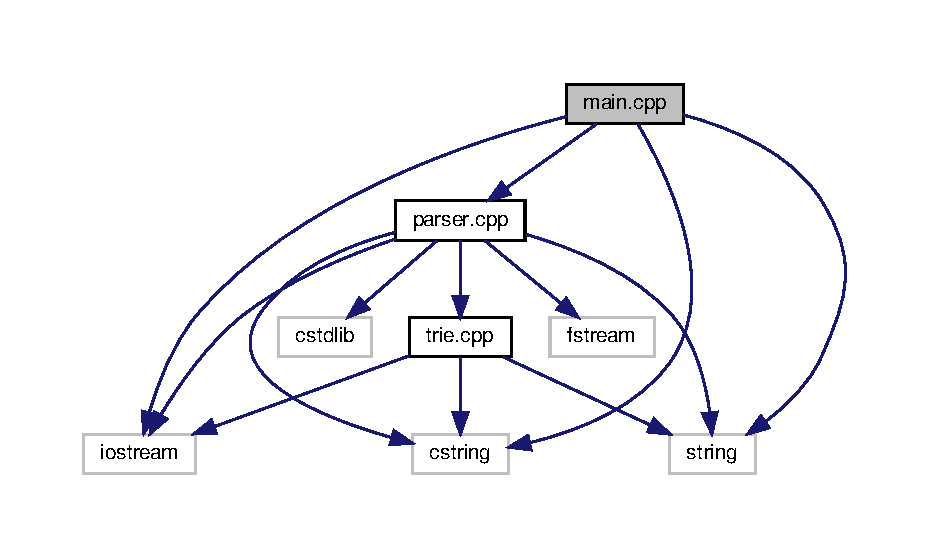
\includegraphics[width=350pt]{main_8cpp__incl}
\end{center}
\end{figure}
\subsection*{Classes}
\begin{DoxyCompactItemize}
\item 
class \hyperlink{classstructures_1_1ElementToSee}{structures\+::\+Element\+To\+See}
\end{DoxyCompactItemize}
\subsection*{Namespaces}
\begin{DoxyCompactItemize}
\item 
 \hyperlink{namespacestructures}{structures}
\begin{DoxyCompactList}\small\item\em Copyright 2018 Maria Eduarda de Melo Hang. \end{DoxyCompactList}\end{DoxyCompactItemize}
\subsection*{Functions}
\begin{DoxyCompactItemize}
\item 
std\+::string \hyperlink{main_8cpp_ad7ad8d67f833642b881180a9ba81e15f}{get\+X\+M\+L\+Text} (char xmlfilename\mbox{[}$\,$\mbox{]})
\begin{DoxyCompactList}\small\item\em Leitura do arquivo xml e armazenamento do respectivo texto. \end{DoxyCompactList}\item 
int \hyperlink{main_8cpp_af3e43fb298e5b8f503703685dfc23d23}{counting\+Width\+Tags} (std\+::string X\+M\+Ltext)
\begin{DoxyCompactList}\small\item\em Contagem das tags \char`\"{}$<$width$>$\char`\"{}. \end{DoxyCompactList}\item 
int \hyperlink{main_8cpp_af2b59f8887b5a6bf75d4666b00e4815d}{counting\+Height\+Tags} (std\+::string X\+M\+Ltext)
\begin{DoxyCompactList}\small\item\em Contagem das tags \char`\"{}$<$height$>$\char`\"{}. \end{DoxyCompactList}\item 
int \hyperlink{main_8cpp_a8371bf9943c9d71d1edd5f635fc6e7ac}{counting\+Name\+Tags} (std\+::string X\+M\+Ltext)
\begin{DoxyCompactList}\small\item\em Contagem das tags \char`\"{}$<$name$>$\char`\"{}. \end{DoxyCompactList}\item 
bool \hyperlink{main_8cpp_aab70c8c83c6f2052ae314fca46147f1b}{find\+The\+Begin\+Of\+X\+ML} (std\+::string X\+M\+Ltext)
\begin{DoxyCompactList}\small\item\em Verificação da existência da tag \char`\"{}$<$dataset$>$\char`\"{}. \end{DoxyCompactList}\item 
bool \hyperlink{main_8cpp_ab00b42e16b61b25a9ed03a75fad135b4}{find\+The\+End\+Of\+X\+ML} (std\+::string X\+M\+Ltext)
\begin{DoxyCompactList}\small\item\em Verificação da existência da tag \char`\"{}$<$/dataset$>$\char`\"{}. \end{DoxyCompactList}\item 
int \hyperlink{main_8cpp_a99c00fc658e4cfb7b88e1264cac634fd}{look\+Up} (int $\ast$$\ast$matrix, int line, int column)
\begin{DoxyCompactList}\small\item\em Verificando o elemento acima do elemento referência. \end{DoxyCompactList}\item 
int $\ast$$\ast$ \hyperlink{main_8cpp_a11b33dfaa6c3264f70269f2f960bda30}{create\+Matrix\+Base} (int lines, int columns)
\begin{DoxyCompactList}\small\item\em Criação de uma matriz nula. \end{DoxyCompactList}\item 
int \hyperlink{main_8cpp_ad4d269b04f7a3e03c4ba9c4590f668c5}{look\+Left} (int $\ast$$\ast$matrix, int line, int column)
\begin{DoxyCompactList}\small\item\em Verificando o elemento à esquerda do elemento referência. \end{DoxyCompactList}\item 
std\+::string \hyperlink{main_8cpp_aeea16cc55e03e11286d0f67377546246}{cleaning\+Matrix\+String} (std\+::string string\+Matrix)
\begin{DoxyCompactList}\small\item\em Retirada do caractere de quebra de linha das strings das matrizes. \end{DoxyCompactList}\item 
int $\ast$ \hyperlink{main_8cpp_a93f0aeb2b15fbc361118a08869d71c80}{get\+Matrix\+Widths} (std\+::string X\+M\+Ltext, int count\+Widths)
\begin{DoxyCompactList}\small\item\em Extração das colunas das matrizes. \end{DoxyCompactList}\item 
std\+::string $\ast$ \hyperlink{main_8cpp_a5641cbfa268d04ca53d7455517a65f78}{get\+X\+M\+L\+Matrix} (std\+::string X\+M\+Ltext, int counter)
\begin{DoxyCompactList}\small\item\em Extração das matrizes. \end{DoxyCompactList}\item 
int $\ast$ \hyperlink{main_8cpp_a883198d3926ad62b7dedc590e66a3197}{get\+Matrix\+Heights} (std\+::string X\+M\+Ltext, int count\+Heights)
\begin{DoxyCompactList}\small\item\em Extração das linhas das matrizes. \end{DoxyCompactList}\item 
int \hyperlink{main_8cpp_a93f55add296e10462fb0a492afc81197}{look\+Down} (int $\ast$$\ast$matrix, int line, int column, int lines)
\begin{DoxyCompactList}\small\item\em Verificando o elemento abaixo do elemento referência. \end{DoxyCompactList}\item 
int \hyperlink{main_8cpp_a5af6beed6446499ed739f7dac94025be}{look\+Right} (int $\ast$$\ast$matrix, int line, int column, int columns)
\begin{DoxyCompactList}\small\item\em Verificando o elemento à direita do elemento referência. \end{DoxyCompactList}\item 
std\+::string $\ast$ \hyperlink{main_8cpp_a0fad19e1d327b8b2a573dd7d77aa505c}{getting\+Image\+Names} (std\+::string X\+M\+Ltext, int count\+Names)
\begin{DoxyCompactList}\small\item\em Extração dos nomes das imagens. \end{DoxyCompactList}\item 
int $\ast$$\ast$ \hyperlink{main_8cpp_ad312896100129e8be16d90ce24da2691}{transform\+To\+Int\+Matrix} (std\+::string string\+Matrix, int lines, int columns)
\begin{DoxyCompactList}\small\item\em Transformação das matrizes do arquivo xml em matrizes inteiras. \end{DoxyCompactList}\item 
void \hyperlink{main_8cpp_a78ee5a2a627636054ba235d1018c06d5}{parsing\+X\+ML} (std\+::string X\+M\+Ltext, \hyperlink{classstructures_1_1LinkedStack}{structures\+::\+Linked\+Stack}$<$ std\+::string $>$ stack\+To\+Tags)
\begin{DoxyCompactList}\small\item\em Verificação dos fechamentos das tags no arquivo xml. \end{DoxyCompactList}\item 
int \hyperlink{main_8cpp_a3c7abfa5a300162f8080613a4dfc054c}{search\+Matrix} (int $\ast$$\ast$matrix\+X\+ML, int $\ast$$\ast$matrix\+Auxiliar, int lines, int columns, \hyperlink{classstructures_1_1LinkedQueue}{structures\+::\+Linked\+Queue}$<$ \hyperlink{classstructures_1_1ElementToSee}{structures\+::\+Element\+To\+See} $>$ elements\+Queue)
\begin{DoxyCompactList}\small\item\em Rotulamento da Matriz (vizinhança 4). \end{DoxyCompactList}\item 
int \hyperlink{main_8cpp_ae66f6b31b5ad750f1fe042a706a4e3d4}{main} ()
\begin{DoxyCompactList}\small\item\em Recebe o nome do arquivo como entrada e chama todos os metodos necessarios. \end{DoxyCompactList}\end{DoxyCompactItemize}


\subsection{Detailed Description}
Primeiro trabalho da disciplina de Estrutura de Dados(\+I\+N\+E5408). 

Propósito\+: Verificação do fechamento de \char`\"{}tags\char`\"{} no arquivo xml mediante uma pilha encadeada de strings e rotulação das imagens binárias, presentes no segmento \char`\"{}$<$data$>$\char`\"{}, com o uso de vizinhança 4, utilizando duas filas encadeadas contendo\+: matrizes inteiras e Element\+To\+See (struct definida).

\begin{DoxyAuthor}{Author}
Maria Eduarda de Melo Hang 
\end{DoxyAuthor}
\begin{DoxyDate}{Date}
06 October 2018 
\end{DoxyDate}


\subsection{Function Documentation}
\mbox{\Hypertarget{main_8cpp_aeea16cc55e03e11286d0f67377546246}\label{main_8cpp_aeea16cc55e03e11286d0f67377546246}} 
\index{main.\+cpp@{main.\+cpp}!cleaning\+Matrix\+String@{cleaning\+Matrix\+String}}
\index{cleaning\+Matrix\+String@{cleaning\+Matrix\+String}!main.\+cpp@{main.\+cpp}}
\subsubsection{\texorpdfstring{cleaning\+Matrix\+String()}{cleaningMatrixString()}}
{\footnotesize\ttfamily std\+::string cleaning\+Matrix\+String (\begin{DoxyParamCaption}\item[{std\+::string}]{string\+Matrix }\end{DoxyParamCaption})}



Retirada do caractere de quebra de linha das strings das matrizes. 

Caso o caractere de quebra de linha seja encontrado nessa string, será pego o índice e removido com o uso do método erase até que não reste mais nenhum.


\begin{DoxyParams}{Parameters}
{\em string\+Matrix} & A string que contém uma das matrizes do arquivo xml. \\
\hline
\end{DoxyParams}
\begin{DoxyReturn}{Returns}
Uma string sem o caractere de quebra de linha presente. 
\end{DoxyReturn}
\mbox{\Hypertarget{main_8cpp_af2b59f8887b5a6bf75d4666b00e4815d}\label{main_8cpp_af2b59f8887b5a6bf75d4666b00e4815d}} 
\index{main.\+cpp@{main.\+cpp}!counting\+Height\+Tags@{counting\+Height\+Tags}}
\index{counting\+Height\+Tags@{counting\+Height\+Tags}!main.\+cpp@{main.\+cpp}}
\subsubsection{\texorpdfstring{counting\+Height\+Tags()}{countingHeightTags()}}
{\footnotesize\ttfamily int counting\+Height\+Tags (\begin{DoxyParamCaption}\item[{std\+::string}]{X\+M\+Ltext }\end{DoxyParamCaption})}



Contagem das tags \char`\"{}$<$height$>$\char`\"{}. 

Ao encontrar a tag \char`\"{}$<$height$>$\char`\"{}, o contador será incrementado.


\begin{DoxyParams}{Parameters}
{\em X\+M\+Ltext} & A string que contém o texto arquivo xml. \\
\hline
\end{DoxyParams}
\begin{DoxyReturn}{Returns}
Um inteiro representando a quantidade de tags \char`\"{}$<$height$>$\char`\"{} encontradas. 
\end{DoxyReturn}
\mbox{\Hypertarget{main_8cpp_a8371bf9943c9d71d1edd5f635fc6e7ac}\label{main_8cpp_a8371bf9943c9d71d1edd5f635fc6e7ac}} 
\index{main.\+cpp@{main.\+cpp}!counting\+Name\+Tags@{counting\+Name\+Tags}}
\index{counting\+Name\+Tags@{counting\+Name\+Tags}!main.\+cpp@{main.\+cpp}}
\subsubsection{\texorpdfstring{counting\+Name\+Tags()}{countingNameTags()}}
{\footnotesize\ttfamily int counting\+Name\+Tags (\begin{DoxyParamCaption}\item[{std\+::string}]{X\+M\+Ltext }\end{DoxyParamCaption})}



Contagem das tags \char`\"{}$<$name$>$\char`\"{}. 

Ao encontrar a tag \char`\"{}$<$name$>$\char`\"{}, o contador será incrementado.


\begin{DoxyParams}{Parameters}
{\em X\+M\+Ltext} & A string que contém o texto arquivo xml. \\
\hline
\end{DoxyParams}
\begin{DoxyReturn}{Returns}
Um inteiro representando a quantidade de tags \char`\"{}$<$name$>$\char`\"{} encontradas. 
\end{DoxyReturn}
\mbox{\Hypertarget{main_8cpp_af3e43fb298e5b8f503703685dfc23d23}\label{main_8cpp_af3e43fb298e5b8f503703685dfc23d23}} 
\index{main.\+cpp@{main.\+cpp}!counting\+Width\+Tags@{counting\+Width\+Tags}}
\index{counting\+Width\+Tags@{counting\+Width\+Tags}!main.\+cpp@{main.\+cpp}}
\subsubsection{\texorpdfstring{counting\+Width\+Tags()}{countingWidthTags()}}
{\footnotesize\ttfamily int counting\+Width\+Tags (\begin{DoxyParamCaption}\item[{std\+::string}]{X\+M\+Ltext }\end{DoxyParamCaption})}



Contagem das tags \char`\"{}$<$width$>$\char`\"{}. 

Ao encontrar a tag \char`\"{}$<$width$>$\char`\"{}, o contador será incrementado.


\begin{DoxyParams}{Parameters}
{\em X\+M\+Ltext} & A string que contém o texto arquivo xml. \\
\hline
\end{DoxyParams}
\begin{DoxyReturn}{Returns}
Um inteiro representando a quantidade de tags \char`\"{}$<$width$>$\char`\"{} encontradas. 
\end{DoxyReturn}
\mbox{\Hypertarget{main_8cpp_a11b33dfaa6c3264f70269f2f960bda30}\label{main_8cpp_a11b33dfaa6c3264f70269f2f960bda30}} 
\index{main.\+cpp@{main.\+cpp}!create\+Matrix\+Base@{create\+Matrix\+Base}}
\index{create\+Matrix\+Base@{create\+Matrix\+Base}!main.\+cpp@{main.\+cpp}}
\subsubsection{\texorpdfstring{create\+Matrix\+Base()}{createMatrixBase()}}
{\footnotesize\ttfamily int $\ast$$\ast$ create\+Matrix\+Base (\begin{DoxyParamCaption}\item[{int}]{lines,  }\item[{int}]{columns }\end{DoxyParamCaption})}



Criação de uma matriz nula. 

Cria uma matriz nula para ser usada na rotulação, tendo a mesma quantidade de linhas e colunas que matriz do xml.


\begin{DoxyParams}{Parameters}
{\em lines} & Quantiade de linhas. \\
\hline
{\em columns} & Quantidade de colunas. \\
\hline
\end{DoxyParams}
\begin{DoxyReturn}{Returns}
Uma matriz de inteiros nula. 
\end{DoxyReturn}
\mbox{\Hypertarget{main_8cpp_aab70c8c83c6f2052ae314fca46147f1b}\label{main_8cpp_aab70c8c83c6f2052ae314fca46147f1b}} 
\index{main.\+cpp@{main.\+cpp}!find\+The\+Begin\+Of\+X\+ML@{find\+The\+Begin\+Of\+X\+ML}}
\index{find\+The\+Begin\+Of\+X\+ML@{find\+The\+Begin\+Of\+X\+ML}!main.\+cpp@{main.\+cpp}}
\subsubsection{\texorpdfstring{find\+The\+Begin\+Of\+X\+M\+L()}{findTheBeginOfXML()}}
{\footnotesize\ttfamily bool find\+The\+Begin\+Of\+X\+ML (\begin{DoxyParamCaption}\item[{std\+::string}]{X\+M\+Ltext }\end{DoxyParamCaption})}



Verificação da existência da tag \char`\"{}$<$dataset$>$\char`\"{}. 

Esse método, com a utilização do método find, procurará pela tag \char`\"{}$<$dataset$>$\char`\"{}, caso seja encontrada, será atribuído o índice onde se encontra e retornará verdadeiro. Caso contrário, retornará falso.


\begin{DoxyParams}{Parameters}
{\em X\+M\+Ltext} & A string que contém o texto arquivo xml. \\
\hline
\end{DoxyParams}
\begin{DoxyReturn}{Returns}
Retornará verdadeiro se a tag \char`\"{}$<$dataset$>$\char`\"{} foi encontrada no arquivo. 
\end{DoxyReturn}
\mbox{\Hypertarget{main_8cpp_ab00b42e16b61b25a9ed03a75fad135b4}\label{main_8cpp_ab00b42e16b61b25a9ed03a75fad135b4}} 
\index{main.\+cpp@{main.\+cpp}!find\+The\+End\+Of\+X\+ML@{find\+The\+End\+Of\+X\+ML}}
\index{find\+The\+End\+Of\+X\+ML@{find\+The\+End\+Of\+X\+ML}!main.\+cpp@{main.\+cpp}}
\subsubsection{\texorpdfstring{find\+The\+End\+Of\+X\+M\+L()}{findTheEndOfXML()}}
{\footnotesize\ttfamily bool find\+The\+End\+Of\+X\+ML (\begin{DoxyParamCaption}\item[{std\+::string}]{X\+M\+Ltext }\end{DoxyParamCaption})}



Verificação da existência da tag \char`\"{}$<$/dataset$>$\char`\"{}. 

Esse método, com a utilização do método find, procurará pela tag \char`\"{}$<$/dataset$>$\char`\"{}, caso seja encontrada, será atribuído o índice onde se encontra e retornará verdadeiro. Caso contrário, retornará falso.


\begin{DoxyParams}{Parameters}
{\em X\+M\+Ltext} & A string que contém o texto arquivo xml. \\
\hline
\end{DoxyParams}
\begin{DoxyReturn}{Returns}
Retornará verdadeiro se a tag \char`\"{}$<$/dataset$>$\char`\"{} foi encontrada no arquivo. 
\end{DoxyReturn}
\mbox{\Hypertarget{main_8cpp_a883198d3926ad62b7dedc590e66a3197}\label{main_8cpp_a883198d3926ad62b7dedc590e66a3197}} 
\index{main.\+cpp@{main.\+cpp}!get\+Matrix\+Heights@{get\+Matrix\+Heights}}
\index{get\+Matrix\+Heights@{get\+Matrix\+Heights}!main.\+cpp@{main.\+cpp}}
\subsubsection{\texorpdfstring{get\+Matrix\+Heights()}{getMatrixHeights()}}
{\footnotesize\ttfamily int $\ast$ get\+Matrix\+Heights (\begin{DoxyParamCaption}\item[{std\+::string}]{X\+M\+Ltext,  }\item[{int}]{count\+Heights }\end{DoxyParamCaption})}



Extração das linhas das matrizes. 

Da mesma forma que o método parsing\+X\+ML, utiliza-\/se a função find da biblioteca de strings, nesse caso as strings padrão serão \char`\"{}$<$height$>$\char`\"{}, para obter o índice do primeiro caractere, e \char`\"{}$<$/height$>$\char`\"{}, para encontrar o índice do último caractere dessa tag. Posteriormente, será pego a substring presente no intervalo \mbox{[}begin, position -\/ begin\mbox{]}, sendo extraído apenas o número entre as duas tags. Por fim, essa substring será convertida em inteiro e guardada no array de inteiros heights. O begin será incrementado para buscar os novos índices.


\begin{DoxyParams}{Parameters}
{\em X\+M\+Ltext} & A string que contém o texto arquivo xml. \\
\hline
{\em count\+Heights} & Quantidade de valores que devem ser coletados da string(número de matrizes presentes no arquivo). \\
\hline
\end{DoxyParams}
\begin{DoxyReturn}{Returns}
Um array de inteiros contendo todos os valores de linhas de cada matriz contida no arquivo xml. 
\end{DoxyReturn}
\mbox{\Hypertarget{main_8cpp_a93f0aeb2b15fbc361118a08869d71c80}\label{main_8cpp_a93f0aeb2b15fbc361118a08869d71c80}} 
\index{main.\+cpp@{main.\+cpp}!get\+Matrix\+Widths@{get\+Matrix\+Widths}}
\index{get\+Matrix\+Widths@{get\+Matrix\+Widths}!main.\+cpp@{main.\+cpp}}
\subsubsection{\texorpdfstring{get\+Matrix\+Widths()}{getMatrixWidths()}}
{\footnotesize\ttfamily int $\ast$ get\+Matrix\+Widths (\begin{DoxyParamCaption}\item[{std\+::string}]{X\+M\+Ltext,  }\item[{int}]{count\+Widths }\end{DoxyParamCaption})}



Extração das colunas das matrizes. 

Da mesma forma que o método parsing\+X\+ML, utiliza-\/se a função find da biblioteca de strings, nesse caso as strings padrão serão \char`\"{}$<$width$>$\char`\"{}, para obter o índice do primeiro caractere, e \char`\"{}$<$/width$>$\char`\"{}, para encontrar o índice do último caractere dessa tag. Posteriormente, será pego a substring presente no intervalo \mbox{[}begin, position -\/ begin\mbox{]}, sendo extraído apenas o número entre as duas tags. Por fim, essa substring será convertida em inteiro e guardada no array de inteiros widths. O begin será incrementado para buscar os novos índices.


\begin{DoxyParams}{Parameters}
{\em X\+M\+Ltext} & A string que contém o texto arquivo xml. \\
\hline
{\em count\+Widths} & Quantidade de valores que devem ser coletados da string(número de matrizes presentes no arquivo). \\
\hline
\end{DoxyParams}
\begin{DoxyReturn}{Returns}
Um array de inteiros contendo todos os valores de colunas de cada matriz contida no arquivo xml. 
\end{DoxyReturn}
\mbox{\Hypertarget{main_8cpp_a0fad19e1d327b8b2a573dd7d77aa505c}\label{main_8cpp_a0fad19e1d327b8b2a573dd7d77aa505c}} 
\index{main.\+cpp@{main.\+cpp}!getting\+Image\+Names@{getting\+Image\+Names}}
\index{getting\+Image\+Names@{getting\+Image\+Names}!main.\+cpp@{main.\+cpp}}
\subsubsection{\texorpdfstring{getting\+Image\+Names()}{gettingImageNames()}}
{\footnotesize\ttfamily std\+::string $\ast$ getting\+Image\+Names (\begin{DoxyParamCaption}\item[{std\+::string}]{X\+M\+Ltext,  }\item[{int}]{count\+Names }\end{DoxyParamCaption})}



Extração dos nomes das imagens. 

Da mesma forma que o método parsing\+X\+ML, utiliza-\/se a função find da biblioteca de strings, nesse caso as strings padrão serão \char`\"{}$<$name$>$\char`\"{}, para obter o índice do primeiro caractere, e \char`\"{}$<$/name$>$\char`\"{}, para encontrar o índice do último caractere dessa tag. Posteriormente, será pego a substring presente no intervalo \mbox{[}begin, position -\/ begin\mbox{]}, sendo extraído apenas o número entre as duas tags. Por fim, essa substring será guardada no array de strings names. O begin será incrementado para buscar os novos índices.


\begin{DoxyParams}{Parameters}
{\em X\+M\+Ltext} & A string que contém o texto arquivo xml. \\
\hline
{\em count\+Names} & Quantidade de nomes que devem ser buscados. \\
\hline
\end{DoxyParams}
\begin{DoxyReturn}{Returns}
Um array de strings contendo todos os nomes das imagens. 
\end{DoxyReturn}
\mbox{\Hypertarget{main_8cpp_a5641cbfa268d04ca53d7455517a65f78}\label{main_8cpp_a5641cbfa268d04ca53d7455517a65f78}} 
\index{main.\+cpp@{main.\+cpp}!get\+X\+M\+L\+Matrix@{get\+X\+M\+L\+Matrix}}
\index{get\+X\+M\+L\+Matrix@{get\+X\+M\+L\+Matrix}!main.\+cpp@{main.\+cpp}}
\subsubsection{\texorpdfstring{get\+X\+M\+L\+Matrix()}{getXMLMatrix()}}
{\footnotesize\ttfamily std\+::string $\ast$ get\+X\+M\+L\+Matrix (\begin{DoxyParamCaption}\item[{std\+::string}]{X\+M\+Ltext,  }\item[{int}]{counter }\end{DoxyParamCaption})}



Extração das matrizes. 

Da mesma forma que nos métodos de extração de linhas e colunas das matrizes, esse método realizará a busca das matrizes contidas entre as tags com o padrão \char`\"{}$<$data$>$\char`\"{} e \char`\"{}$<$/data$>$\char`\"{}, pegando os respectivos índices e extraindo a substring no intervalo \mbox{[}begin, position -\/ begin\mbox{]} (a matriz). O begin será incrementado para buscar os novos índices.


\begin{DoxyParams}{Parameters}
{\em X\+M\+Ltext} & A string que contém o texto arquivo xml. \\
\hline
{\em counter} & Quantidade de matrizes presentes no arquivo. \\
\hline
\end{DoxyParams}
\begin{DoxyReturn}{Returns}
Um array de strings contendo cada matrize do arquivo xml. 
\end{DoxyReturn}
\mbox{\Hypertarget{main_8cpp_ad7ad8d67f833642b881180a9ba81e15f}\label{main_8cpp_ad7ad8d67f833642b881180a9ba81e15f}} 
\index{main.\+cpp@{main.\+cpp}!get\+X\+M\+L\+Text@{get\+X\+M\+L\+Text}}
\index{get\+X\+M\+L\+Text@{get\+X\+M\+L\+Text}!main.\+cpp@{main.\+cpp}}
\subsubsection{\texorpdfstring{get\+X\+M\+L\+Text()}{getXMLText()}}
{\footnotesize\ttfamily std\+::string get\+X\+M\+L\+Text (\begin{DoxyParamCaption}\item[{char}]{xmlfilename\mbox{[}$\,$\mbox{]} }\end{DoxyParamCaption})}



Leitura do arquivo xml e armazenamento do respectivo texto. 

Primeiramente, tenta-\/se abrir o arquivo xml recebido no terminal, caso não seja possível, o programa sairá retorna 1 (erro). Após essa verificação, o ifstream source lerá caractere por caractere e concatenará com a variável local X\+M\+Ltext e terminará quando encontrar o E\+OF.


\begin{DoxyParams}{Parameters}
{\em xmlfilename} & Nome do arquivo xml que será aberto e lido. \\
\hline
\end{DoxyParams}
\begin{DoxyReturn}{Returns}
O texto do arquivo xml em formate de uma string. 
\end{DoxyReturn}
\mbox{\Hypertarget{main_8cpp_a93f55add296e10462fb0a492afc81197}\label{main_8cpp_a93f55add296e10462fb0a492afc81197}} 
\index{main.\+cpp@{main.\+cpp}!look\+Down@{look\+Down}}
\index{look\+Down@{look\+Down}!main.\+cpp@{main.\+cpp}}
\subsubsection{\texorpdfstring{look\+Down()}{lookDown()}}
{\footnotesize\ttfamily int look\+Down (\begin{DoxyParamCaption}\item[{int $\ast$$\ast$}]{matrix,  }\item[{int}]{line,  }\item[{int}]{column,  }\item[{int}]{lines }\end{DoxyParamCaption})}



Verificando o elemento abaixo do elemento referência. 


\begin{DoxyParams}{Parameters}
{\em matrix} & A matriz. \\
\hline
{\em line} & A linha do elemento de referência que deseja verificar. \\
\hline
{\em column} & A coluna do elemento de referência que deseja verificar. \\
\hline
{\em lines} & Quantidade de linhas da matriz para testar o limite do índice. \\
\hline
\end{DoxyParams}
\begin{DoxyReturn}{Returns}
Retornará 1 caso o elemento debaixo contenha o valor 1, caso contrário, 0. 
\end{DoxyReturn}
\mbox{\Hypertarget{main_8cpp_ad4d269b04f7a3e03c4ba9c4590f668c5}\label{main_8cpp_ad4d269b04f7a3e03c4ba9c4590f668c5}} 
\index{main.\+cpp@{main.\+cpp}!look\+Left@{look\+Left}}
\index{look\+Left@{look\+Left}!main.\+cpp@{main.\+cpp}}
\subsubsection{\texorpdfstring{look\+Left()}{lookLeft()}}
{\footnotesize\ttfamily int look\+Left (\begin{DoxyParamCaption}\item[{int $\ast$$\ast$}]{matrix,  }\item[{int}]{line,  }\item[{int}]{column }\end{DoxyParamCaption})}



Verificando o elemento à esquerda do elemento referência. 


\begin{DoxyParams}{Parameters}
{\em matrix} & A matriz. \\
\hline
{\em line} & A linha do elemento de referência que deseja verificar. \\
\hline
{\em column} & A coluna do elemento de referência que deseja verificar. \\
\hline
\end{DoxyParams}
\begin{DoxyReturn}{Returns}
Retornará 1 caso o elemento à esquerda contenha o valor 1, caso contrário, 0. 
\end{DoxyReturn}
\mbox{\Hypertarget{main_8cpp_a5af6beed6446499ed739f7dac94025be}\label{main_8cpp_a5af6beed6446499ed739f7dac94025be}} 
\index{main.\+cpp@{main.\+cpp}!look\+Right@{look\+Right}}
\index{look\+Right@{look\+Right}!main.\+cpp@{main.\+cpp}}
\subsubsection{\texorpdfstring{look\+Right()}{lookRight()}}
{\footnotesize\ttfamily int look\+Right (\begin{DoxyParamCaption}\item[{int $\ast$$\ast$}]{matrix,  }\item[{int}]{line,  }\item[{int}]{column,  }\item[{int}]{columns }\end{DoxyParamCaption})}



Verificando o elemento à direita do elemento referência. 


\begin{DoxyParams}{Parameters}
{\em matrix} & A matriz. \\
\hline
{\em line} & A linha do elemento de referência que deseja verificar. \\
\hline
{\em column} & A coluna do elemento de referência que deseja verificar. \\
\hline
{\em columns} & Quantidade de colunas da matriz para testar o limite do índice. \\
\hline
\end{DoxyParams}
\begin{DoxyReturn}{Returns}
Retornará 1 caso o elemento à direita contenha o valor 1, caso contrário, 0. 
\end{DoxyReturn}
\mbox{\Hypertarget{main_8cpp_a99c00fc658e4cfb7b88e1264cac634fd}\label{main_8cpp_a99c00fc658e4cfb7b88e1264cac634fd}} 
\index{main.\+cpp@{main.\+cpp}!look\+Up@{look\+Up}}
\index{look\+Up@{look\+Up}!main.\+cpp@{main.\+cpp}}
\subsubsection{\texorpdfstring{look\+Up()}{lookUp()}}
{\footnotesize\ttfamily int look\+Up (\begin{DoxyParamCaption}\item[{int $\ast$$\ast$}]{matrix,  }\item[{int}]{line,  }\item[{int}]{column }\end{DoxyParamCaption})}



Verificando o elemento acima do elemento referência. 


\begin{DoxyParams}{Parameters}
{\em matrix} & A matriz. \\
\hline
{\em line} & A linha do elemento de referência que deseja verificar. \\
\hline
{\em column} & A coluna do elemento de referência que deseja verificar. \\
\hline
\end{DoxyParams}
\begin{DoxyReturn}{Returns}
Retornará 1 caso o elemento acima contenha o valor 1, caso contrário, 0. 
\end{DoxyReturn}
\mbox{\Hypertarget{main_8cpp_ae66f6b31b5ad750f1fe042a706a4e3d4}\label{main_8cpp_ae66f6b31b5ad750f1fe042a706a4e3d4}} 
\index{main.\+cpp@{main.\+cpp}!main@{main}}
\index{main@{main}!main.\+cpp@{main.\+cpp}}
\subsubsection{\texorpdfstring{main()}{main()}}
{\footnotesize\ttfamily int main (\begin{DoxyParamCaption}{ }\end{DoxyParamCaption})}



Recebe o nome do arquivo como entrada e chama todos os metodos necessarios. 

\mbox{\Hypertarget{main_8cpp_a78ee5a2a627636054ba235d1018c06d5}\label{main_8cpp_a78ee5a2a627636054ba235d1018c06d5}} 
\index{main.\+cpp@{main.\+cpp}!parsing\+X\+ML@{parsing\+X\+ML}}
\index{parsing\+X\+ML@{parsing\+X\+ML}!main.\+cpp@{main.\+cpp}}
\subsubsection{\texorpdfstring{parsing\+X\+M\+L()}{parsingXML()}}
{\footnotesize\ttfamily void parsing\+X\+ML (\begin{DoxyParamCaption}\item[{std\+::string}]{X\+M\+Ltext,  }\item[{\hyperlink{classstructures_1_1LinkedStack}{structures\+::\+Linked\+Stack}$<$ std\+::string $>$}]{stack\+To\+Tags }\end{DoxyParamCaption})}



Verificação dos fechamentos das tags no arquivo xml. 

Usando o método find da biblioteca de strings, pegará o índice do primeiro caractere que for igual a \char`\"{}$<$\char`\"{}, depois o outro índice que for igual a \char`\"{}$>$\char`\"{} e por fim pegará uma substring, presente no intervalo \mbox{[}begin, end -\/ begin + 1\mbox{]} do texto do X\+ML e passará para a string auxiliar. Caso o caractere \char`\"{}/\char`\"{} seja encontrado, ele será retirado com o método erase. Posteriormente, haverá uma verificação no caso da pilha ser vazia, se a condição for verdadeira, essa string auxiliar será automaticamente empilhada. Caso contrário, o método verificará se o topo coincide com a string auxiliar, se for verdade, a pilha realizará um pop, caso contrário um push, colocando a auxiliar como parâmetro. Ao fim, o begin será incrementado para pegar o próximo índice do caractere que conter o \char`\"{}$<$\char`\"{}. Caso uma tag de fechamento foi encontrada e não for igual ao topo, o programa será finalizado e colocará \char`\"{}error\char`\"{} na tela.


\begin{DoxyParams}{Parameters}
{\em X\+M\+Ltext} & A string que contém o texto arquivo xml. \\
\hline
{\em stack\+To\+Tags} & Uma pilha para guardar as tags. \\
\hline
\end{DoxyParams}
\mbox{\Hypertarget{main_8cpp_a3c7abfa5a300162f8080613a4dfc054c}\label{main_8cpp_a3c7abfa5a300162f8080613a4dfc054c}} 
\index{main.\+cpp@{main.\+cpp}!search\+Matrix@{search\+Matrix}}
\index{search\+Matrix@{search\+Matrix}!main.\+cpp@{main.\+cpp}}
\subsubsection{\texorpdfstring{search\+Matrix()}{searchMatrix()}}
{\footnotesize\ttfamily int search\+Matrix (\begin{DoxyParamCaption}\item[{int $\ast$$\ast$}]{matrix\+X\+ML,  }\item[{int $\ast$$\ast$}]{matrix\+Auxiliar,  }\item[{int}]{lines,  }\item[{int}]{columns,  }\item[{\hyperlink{classstructures_1_1LinkedQueue}{structures\+::\+Linked\+Queue}$<$ \hyperlink{classstructures_1_1ElementToSee}{structures\+::\+Element\+To\+See} $>$}]{elements\+Queue }\end{DoxyParamCaption})}



Rotulamento da Matriz (vizinhança 4). 

Primeiramente, o método percorrerá a matriz do xml e ao encontrar o valor 1 em um dos elementos, ocorrerá uma verificação para ver se já não foi visitado na matriz de rotulamento (se não foi visitado o valor será 0), caso não tenha sido visitado, será instanciado um elemento da classe Element\+To\+See para guardar a linha e coluna desse elemento, sendo inserido na fila de rotulamento, e o rótulo será aplicado aplicado a matriz de rotulamento na mesma linha e coluna. Posteriormente, os 4 vizinhos desse elemento serão verificados com os métodos look\+Up, look\+Down, look\+Right e look\+Left e depois se a matriz de rotulamento já não visitou esse vizinho outro elemento da classe Element\+To\+See será instanciado e inserido na fila de rotulamento e o rótulo atual será atribuído ao vizinho que atendeu às condições mostradas anteriormente. Por fim, o rótulo será incrementado se nenhum outro elemento conexo for encontrado.


\begin{DoxyParams}{Parameters}
{\em matrix\+X\+ML} & A matriz de inteiros do arquivo xml. \\
\hline
{\em matrix\+Auxiliar} & A matriz auxiliar de rotulamento. \\
\hline
{\em lines} & Quantidade de linhas da matriz. \\
\hline
{\em columns} & Quantidade de colunas da matriz. \\
\hline
{\em elements\+Queue} & Fila para guardar os elementos a serem verificados e seus vizinhos (vizinhança 4). \\
\hline
\end{DoxyParams}
\begin{DoxyReturn}{Returns}
O maior rótulo atribuído. 
\end{DoxyReturn}
\mbox{\Hypertarget{main_8cpp_ad312896100129e8be16d90ce24da2691}\label{main_8cpp_ad312896100129e8be16d90ce24da2691}} 
\index{main.\+cpp@{main.\+cpp}!transform\+To\+Int\+Matrix@{transform\+To\+Int\+Matrix}}
\index{transform\+To\+Int\+Matrix@{transform\+To\+Int\+Matrix}!main.\+cpp@{main.\+cpp}}
\subsubsection{\texorpdfstring{transform\+To\+Int\+Matrix()}{transformToIntMatrix()}}
{\footnotesize\ttfamily int $\ast$$\ast$ transform\+To\+Int\+Matrix (\begin{DoxyParamCaption}\item[{std\+::string}]{string\+Matrix,  }\item[{int}]{lines,  }\item[{int}]{columns }\end{DoxyParamCaption})}



Transformação das matrizes do arquivo xml em matrizes inteiras. 

Para realizar essa transformação, o método pegará caractere por caractere e inserir na matriz de inteiros em cada elemento da respectiva posição.


\begin{DoxyParams}{Parameters}
{\em string\+Matrix} & A string que contém uma matriz do arquivo xml. \\
\hline
{\em lines} & Quantidade de linhas da matriz. \\
\hline
{\em columns} & Quantidade de colunas da matriz. \\
\hline
\end{DoxyParams}
\begin{DoxyReturn}{Returns}
Uma matriz de inteiros contendo os valores (0 ou 1) da matrize do arquivo xml. 
\end{DoxyReturn}

\hypertarget{parser_8cpp}{}\section{parser.\+cpp File Reference}
\label{parser_8cpp}\index{parser.\+cpp@{parser.\+cpp}}


Parser dos arquivos dos dicionários.  


{\ttfamily \#include $<$iostream$>$}\newline
{\ttfamily \#include $<$string$>$}\newline
{\ttfamily \#include $<$cstring$>$}\newline
{\ttfamily \#include $<$cstdlib$>$}\newline
{\ttfamily \#include $<$fstream$>$}\newline
{\ttfamily \#include \char`\"{}trie.\+cpp\char`\"{}}\newline
Include dependency graph for parser.\+cpp\+:\nopagebreak
\begin{figure}[H]
\begin{center}
\leavevmode
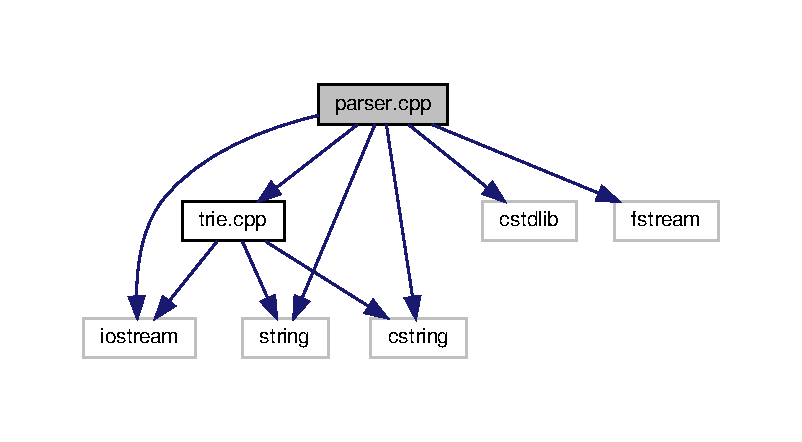
\includegraphics[width=350pt]{parser_8cpp__incl}
\end{center}
\end{figure}
This graph shows which files directly or indirectly include this file\+:
\nopagebreak
\begin{figure}[H]
\begin{center}
\leavevmode
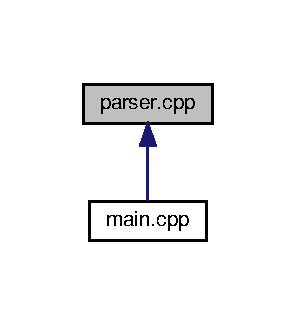
\includegraphics[width=142pt]{parser_8cpp__dep__incl}
\end{center}
\end{figure}
\subsection*{Classes}
\begin{DoxyCompactItemize}
\item 
class \hyperlink{classstructures_1_1Parser}{structures\+::\+Parser}
\end{DoxyCompactItemize}


\subsection{Detailed Description}
Parser dos arquivos dos dicionários. 

\begin{DoxyAuthor}{Author}
Maria Eduarda de Melo Hang 
\end{DoxyAuthor}
\begin{DoxyDate}{Date}
15 November 2018 
\end{DoxyDate}

\hypertarget{trie_8cpp}{}\section{trie.\+cpp File Reference}
\label{trie_8cpp}\index{trie.\+cpp@{trie.\+cpp}}


Árvore de Prefixos que suporta os caracteres de a até z como nodos. Não suporta acentos ou caracteres especiais para a inserção.  


{\ttfamily \#include $<$string$>$}\newline
{\ttfamily \#include $<$cstring$>$}\newline
{\ttfamily \#include $<$iostream$>$}\newline
Include dependency graph for trie.\+cpp\+:\nopagebreak
\begin{figure}[H]
\begin{center}
\leavevmode
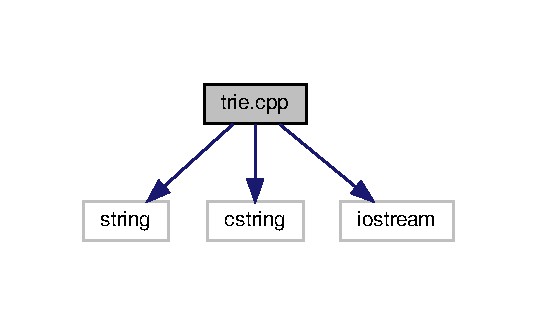
\includegraphics[width=258pt]{trie_8cpp__incl}
\end{center}
\end{figure}
This graph shows which files directly or indirectly include this file\+:
\nopagebreak
\begin{figure}[H]
\begin{center}
\leavevmode
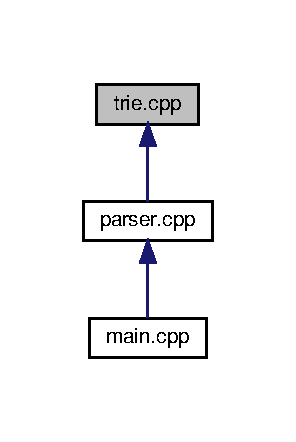
\includegraphics[width=142pt]{trie_8cpp__dep__incl}
\end{center}
\end{figure}
\subsection*{Classes}
\begin{DoxyCompactItemize}
\item 
class \hyperlink{classstructures_1_1Trie}{structures\+::\+Trie}
\begin{DoxyCompactList}\small\item\em Classe da \hyperlink{classstructures_1_1Trie}{Trie}. Estrutura de Dados responsável pela indexação das palavras. \end{DoxyCompactList}\end{DoxyCompactItemize}
\subsection*{Macros}
\begin{DoxyCompactItemize}
\item 
\mbox{\Hypertarget{trie_8cpp_afbca9cff58d15edd9543c3532205d40e}\label{trie_8cpp_afbca9cff58d15edd9543c3532205d40e}} 
\#define {\bfseries S\+T\+R\+U\+C\+T\+U\+R\+E\+S\+\_\+\+T\+R\+I\+E\+\_\+H}
\item 
\#define \hyperlink{trie_8cpp_a97d832ae23af4f215e801e37e4f94254}{K}~26
\end{DoxyCompactItemize}


\subsection{Detailed Description}
Árvore de Prefixos que suporta os caracteres de a até z como nodos. Não suporta acentos ou caracteres especiais para a inserção. 

\begin{DoxyAuthor}{Author}
Maria Eduarda de Melo Hang. 
\end{DoxyAuthor}
\begin{DoxyDate}{Date}
15 November 2018. 
\end{DoxyDate}


\subsection{Macro Definition Documentation}
\mbox{\Hypertarget{trie_8cpp_a97d832ae23af4f215e801e37e4f94254}\label{trie_8cpp_a97d832ae23af4f215e801e37e4f94254}} 
\index{trie.\+cpp@{trie.\+cpp}!K@{K}}
\index{K@{K}!trie.\+cpp@{trie.\+cpp}}
\subsubsection{\texorpdfstring{K}{K}}
{\footnotesize\ttfamily \#define K~26}

constante para guardar a quantidade de caracteres do alfabeto. 
%--- End generated contents ---

% Index
\backmatter
\newpage
\phantomsection
\clearemptydoublepage
\addcontentsline{toc}{chapter}{Index}
\printindex

\end{document}
